\documentclass[tikz,border=3pt]{standalone}
\usepackage[utf8]{inputenc}
\usepackage[T1]{fontenc}
\usepackage{lmodern}
\renewcommand{\familydefault}{\sfdefault}
\usepackage{sansmath}\sansmath
\usepackage{chemfig}
\usepackage{pgfplots}\pgfplotsset{compat=1.18,/pgf/number format/use comma,/pgf/number format/1000 sep={.}}
\usetikzlibrary{arrows.meta,calc,positioning,decorations.pathmorphing,patterns}
% paleta del sitio
\definecolor{nar}{HTML}{E8680C}\definecolor{narc}{HTML}{FFB35C}\definecolor{hielo}{HTML}{FFF3E8}
\definecolor{tinta}{HTML}{1D1D1F}\definecolor{gris}{HTML}{6E6E73}\definecolor{lila}{HTML}{7C5CF0}
\definecolor{azul}{HTML}{2F6FD6}\definecolor{menta}{HTML}{17A673}\definecolor{coral}{HTML}{E8342A}
\begin{document}
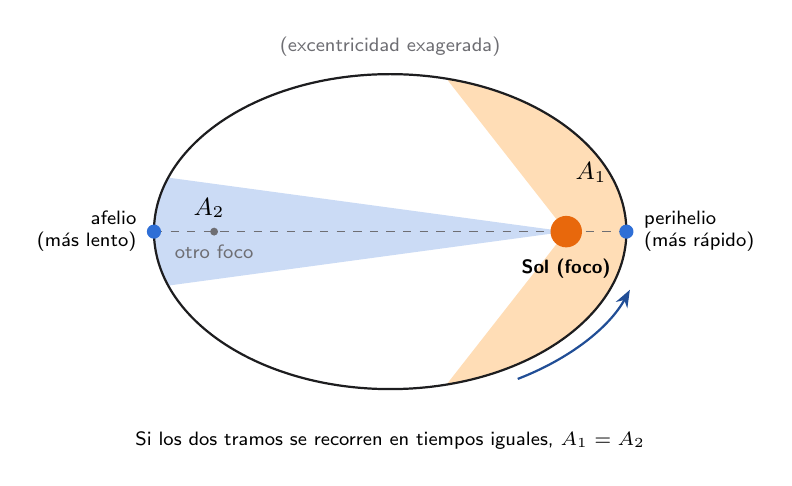
\begin{tikzpicture}[font=\footnotesize,>={Stealth[length=2.2mm]}]
\def\a{3}\def\b{2}\def\c{2.236}
\fill[narc!45] (\c,0) -- plot[domain=-76.2:76.2,samples=60] ({\a*cos(\x)},{\b*sin(\x)}) -- cycle;
\fill[azul!25] (\c,0) -- plot[domain=159.95:200.05,samples=30] ({\a*cos(\x)},{\b*sin(\x)}) -- cycle;
\draw[tinta,thick] (0,0) ellipse (\a cm and \b cm);
\draw[gris,dashed] (-\a,0) -- (\a,0);
\fill[nar] (\c,0) circle (0.2); \node[below=5pt,font=\scriptsize\bfseries] at (\c,-0.05) {Sol (foco)};
\fill[gris] (-\c,0) circle (0.05); \node[below,font=\scriptsize,text=gris] at (-\c,-0.05) {otro foco};
\node[font=\small\bfseries] at (2.55,0.75) {$A_1$};
\node[font=\small\bfseries] at (-2.3,0.3) {$A_2$};
\fill[azul] (\a,0) circle (0.09); \node[right,font=\scriptsize,align=left] at (3.1,0) {perihelio\\(más rápido)};
\fill[azul] (-\a,0) circle (0.09); \node[left,font=\scriptsize,align=right] at (-3.1,0) {afelio\\(más lento)};
\draw[->,thick,azul!70!black] ({1.08*\a*cos(-60)},{1.08*\b*sin(-60)}) arc[start angle=-60,end angle=-20,x radius=1.08*\a cm,y radius=1.08*\b cm];
\node[font=\scriptsize,align=center] at (0,-2.65) {Si los dos tramos se recorren en tiempos iguales, $A_1 = A_2$};
\node[font=\scriptsize,text=gris] at (0,2.35) {(excentricidad exagerada)};
\end{tikzpicture}
\end{document}
